\documentclass[../Kamil_Kowalewski_Main.tex]{subfiles}

\begin{document} {

    Niniejszy rozdział zawiera dokumentację techniczną aplikacji. Jej celem jest
    przedstawienie wszelkich niezbędnych informacji o produkcie, dzięki czemu osoba
    rozpoczynająca rozbudowe lub modyfikację projektu ma możliwość poznania wszystkich
    potrzebnych szczegółów.

    \section{Wymagania funkcjonalne i niefunkcjonalne}
    \label{chapter4:dok_techniczna:wymagania} {

        \subsection{Wymagania funkcjonalne}
        \label{chapter4:dok_techniczna:wymagania:funkc} {
            Wymagania funkcjonalne określają, jakie funkcjonalności ma oferować dany
            system informatyczny, jak ma się zachowywać w~pewnych sytuacjach oraz jak
            ma reagować na charakterystyczne dane wejściowe. Poniżej zostały one
            przedstawione dla aplikacji \textit{Social Racetrack}.

            \noindent\textbf{Wyświetlanie głównej strony}\\
            \indent Strona główna zapewnia użytkownikowi możliwość łatwego dostępu do
            paneli logowania oraz rejestracji użytkownika. Co więcej, zapewniona jest
            informacja o~samym portalu aby zachęcić potencjalnych użytkowników do
            założenia konta.

            \noindent\textbf{Zmiana barw aplikacji}\\
            \indent Użytkownik ma zapewnioną możliwość zmiany barw aplikacji na jasną
            lub ciemną.

            \noindent\textbf{Otwarcie bocznego panelu nawigacyjnego}\\
            \indent Użytkownik ma zapewnioną możliwość otwarcia bocznego panelu
            nawigacyjnego dzięki czemu widoczne są pełne nazwy zamiast samych ikon.

            \noindent\textbf{Rejestracja użytkownika}\\
            \indent Formularz rejestracji użytkownika zapewnia możliwość rejestracji
            z~uprawnieniami zwykłego użytkownika. Minimalny wiek posiadacza konta to 15 lat.

            \noindent\textbf{Logowanie użytkownika}\\
            \indent Formularz logowanie zapewnia użytkownikowi możliwość weryfikacji
            tożsamości, dostępu do konta oraz do funkcjonalności dostępnych dla
            zalogowanych użytkowników, które zostały opisane poniżej.

            \noindent\textbf{Przywracanie hasła użytkownika}\\
            \indent Formularz przywracania hasła zapewnia możliwość użytkownikowi
            anulowania starego hasła i~utworzenie nowego. Opcja ta jest dostępna
            tylko dla użytkowników posiadających konto w~aplikacji oraz mających
            dostęp do poczty email przypisanej do konta, gdyż na tą pocztę jest
            wysyłany link do opisanej powyżej czynności.

            \noindent\textbf{Panel obiektów sportowych}\\
            \indent Panel obiektów sportowych jest dostępny dla użytkownika
            niezalogowanego, zalogowanego oraz administratora. Użytkownik ten ma dostęp
            do wszystkich aktualnie dostępny obiektów sportowych w~aplikacji oraz może
            je wyszukiwać po nazwie.

            \noindent\textbf{Dodawanie obiektu sportowego}\\
            \indent Tylko administrator ma dostępną możliwość dodawania nowego
            obiektu sportowego.

            \noindent\textbf{Podgląd szczegółów obiektu sportowego}\\
            \indent Podgląd szczegółów obiektu sportowego jest dostępny dla użytkownika
            niezalogowanego, zalogowanego oraz administratora. Panel ten zapewnia
            możliwość wyświetlenia użytkownikowi dodatkowych informacji, do których
            należy opis, liczba zakrętów, maksymalna głośność wydechu w~pojeździe oraz
            minimalny prześwit zawieszenia.

            \noindent\textbf{Usuwanie obiektu sportowego}\\
            \indent Tylko administrator ma dostępną możliwość usuwanie istniejącego
            obiektu sportowego.

            \noindent\textbf{Panel konta użytkownika}\\
            \indent Panel konta użytkownika jest dostępny dla danej zalogowanej osoby
            lub administratora. Zapewnia on użytkownikowi możliwość sprawdzenia takich
            informacji jak imię, nazwisko, data ostatniego logowania, adres email do
            tego konta. Użytkownik może obejrzeć flotę pojazdów oraz zdobyte
            osiągnięcia sportowe. Dostępne jest tam również przycisk, dzięki
            któremu można przejść do panelu ustawień konta użytkownika.

            \noindent\textbf{Usuwanie wybranych pojazdów z floty}\\
            \indent Użytkownik może usunąć ze swojego profilu wybrane przez siebie pojazdy
            z~floty.

            \noindent\textbf{Usuwanie wybranych osiągnięć sportowych}\\
            \indent Użytkownik może usunąć ze swojego profilu wybrane przez siebie osiągnięcia
            sportowe.

            \noindent\textbf{Panel ustawień konta użytkownika}\\
            \indent Panel ustawień konta użytkownika jest dostępny dla danej zalogowanej
            osoby lub administratora. Zapewnia on trzy możliwości przedstawione poniżej.

            \noindent\textbf{Dodawanie nowych pojazdów do floty}\\
            \indent Użytkownik zalogowany na swoje konto może dodać nowy pojazd do
            swojej floty.

            \noindent\textbf{Dodawanie nowych osiągnięć sportowych}\\
            \indent Użytkownik zalogowany na swoje konto może dodać nowe
            osiągnięcia sportowe.

            \noindent\textbf{Edycja danych osobowych użytkownika}\\
            \indent Użytkownik zalogowany na swoje konto może edytować swoje
            dane osobowe.

            \noindent\textbf{Usuwanie konta użytkownika}\\
            \indent Usuwanie konta użytkownika w aplikacji jest niemożliwe.

            \noindent\textbf{Tworzenie nowego wydarzenia}\\
            \indent Użytkownik tworzący dane wydarzenie jednocześnie bierze w~nim
            udział. Nie ma możliwości stworzenia wydarzenia i~rezygnacji z~udziału
            w~nim. Tylko administrator ma możliwość usunięcia wydarzenia. Możliwe jest
            utworzenie wydarzenia, którego data jest wcześniejsza niż data utworzenia
            wydarzenie. Skutkuje to automatycznym jego przeniesieniem do wydarzeń
            przeszłych.

            \noindent\textbf{Przeglądanie przyszłych wydarzeń}\\
            \indent Zapewniona jest możliwość przeglądania przyszłych wydarzeń tylko
            dla użytkowników zalogowanych lub ze statusem administratora. Dodatkowo
            użytkownik może je wyszukiwać po nazwie. Gdy do rozpoczęcia wydarzenia
            zostało mniej niż 24 godziny zostanie ono przeniesione do panelu przeszłych
            wydarzeń.

            \noindent\textbf{Przeglądanie przeszłych wydarzeń}\\
            \indent Użytkownik zalogowany lub z~uprawnieniami administratora może
            przeglądać przeszłe wydarzenia. Analogicznie jak w~przypadku przyszłych
            wydarzeń ma on możliwość wyszukiwania ich po nazwie.

            \noindent\textbf{Podgląd szczegółów wydarzenia}\\
            \indent Użytkownik zalogowany lub z~uprawnieniami administratora ma
            możliwość przeglądania szczegółów wszystkich dostępnych wydarzeń.

            \noindent\textbf{Dołączanie do wydarzenia}\\
            \indent Użytkownik, który jest zalogowany lub jest administratorem może
            wziąć udział w~wydarzeniu jeżeli nie jest na liście osób biorących udział.

            \noindent\textbf{Rezygnacja z udziału w wydarzeniu}\\
            \indent Użytkownik, który jest zalogowany lub jest administratorem może
            zrezygnować z~udziału w~wydarzeniu jeżeli dołączył wcześniej do wydarzenia.

            \noindent\textbf{Usuwanie wydarzenia}\\
            \indent Administrator ma możliwość usunięcia wydarzenia. Skutkuje to jego
            usunięciem oraz usunięciem wydarzeń, w których brał lub będzie brał dany
            użytkownik.

            \noindent\textbf{Przeglądanie kont innych użytkowników}\\
            \indent Zapewniona jest możliwość przeglądania kont innych użytkowników tylko
            dla użytkowników zalogowanych lub ze statusem administratora. Dodatkowo
            istnieje możliwość aby użytkownik wyszukiwał konta innych użytkowników
            aplikacji po nazwie.

            \noindent\textbf{Przeglądanie szczegółów kont innych użytkowników}\\
            \indent Użytkownik zalogowany lub z~uprawnieniami administratora ma
            możliwość przeglądania szczegółów wybranego przez niego konta użytkownika.

            \noindent\textbf{Nadawanie uprawnień administratora}\\
            \indent Tylko administrator może nadać uprawnienia administracyjne.
            Wymagane jest aby osoba ta posiadała konta w~aplikacji oraz podała adres
            email, który został podany w~czasie procesu rejestracji. Ten adres email jest
            również wyświetlanych w~panelu konta użytkownika.
        }

        \subsection{Wymagania niefunkcjonalne}
        \label{chapter4:dok_techniczna:wymagania:niefunkc} {
            Wymagania niefunkcjonalne określają ograniczenia przy jakich dany system
            informatyczny ma spełniać swoje funkcje. Poniżej zostały one
            przedstawione dla aplikacji \textit{Social Racetrack}.

            \noindent\textbf{Wysoki stopień bezpieczeństwa}\\
            \indent Zapewnienie wysokiego poziomu bezpieczeństwa w~celu zapewnienia
            poufności danych użytkownika oraz ograniczenie możliwości podszywania
            w~celu wykradnięcia danych lub ich zmiany.

            \noindent\textbf{Łatwość użycia}\\
            \indent Umożliwienie prostego korzystania z~aplikacji, intuicyjnej nauki
            dla osób nie korzystającej z~niej wcześniej oraz schludny i~estetyczny
            wygląd.

            \noindent\textbf{Wysoka wydajność}\\
            \indent Aplikacja powinna działać tak samo dobrze na różnych rodzajach
            urządzeń o zróżnicowanej wydajności. W~przypadku urządzeń zaawansowanych
            technologicznie powinna ona zużywać minimalne ilości zasobów obliczeniowych.

            \noindent\textbf{Modularna architektura aplikacji}\\
            \indent Podział aplikacji na odseparowane moduły, które nie są zależne od
            siebie. Istnieje możliwość podmiany dowolnego z~nich.

            \noindent\textbf{Kompatybilność z popularnymi technologiami}\\
            \indent Aplikacja powinna mieć możliwość działania
            w~technologiach, które są popularne i~wykorzystywane przez większość
            użytkowników sieci Internet.
        }
    }

    \section{Architektura aplikacji}
    \label{chapter4:dok_techniczna:architektura} {
        Aplikacja \textit{Social Racetrack} została stworzona w~koncepcie monolitu.
        Cała logika i~zachowanie aplikacji jest w~jednym miejscu z~podziałem na
        stosowne warstwy. Jest to przeciwieństwo architektury mikroserwisów gdzie
        aplikacja składa się w~wielu małych bloczków czyli małych aplikacji o~zazwyczaj
        jednym zadaniu czy też odpowiedzialności. Przykładem takiego zadania jest
        autentykacja użytkownika. W~przypadku architektury mikroserwisów,
        poszczególne mikroserwisy bardzo często współpracują ze sobą, wymieniając
        między sobą dane.

        Ze względu na dosyć nowatorskie rozwiązanie w~platformie Firebase opisanej
        w~sekcji \ref{chapter3:technologie:firebase} została zastosowana architektura
        monolitu razem ze wzorcem projektowym MVC (ang. Model-View-Controller). Polega
        on na rozdzieleniu aplikacji na trzy warstwy \textit{modelu}, \textit{widoku}
        oraz \textit{kontrolera}, dzięki czemu możliwa jest podmiana komponentu
        umieszczonego w~dowolnej z~trzech warstw na inny kompatybilny komponent. Co
        więcej, baza danych Cloud Firestore, które została opisana w~sekcji
        \ref{chapter3:technologie:firebase:firestore} oraz jej wykorzystanie
        w~aplikacji zostało przedstawione w~sekcji
        \ref{chapter4:dok_techniczna:implementacja:model_danych}, ma dosyć nowatorskie
        podejście gdyż oprócz składowania danych, zapewnia również metody
        CRUD (ang. Create, Read, Update, Delete) do operowania na niej. Z~tego powodu
        w~aplikacji po stronie klienta została stworzona warstwa opakowująca wspomniany
        zestaw metody. Został on dokładnie opisany w~sekcji
        \ref{chapter4:dok_techniczna:implementacja:api}.

        Utworzona dodatkowo warstwa po stronie klienta ma za zadanie ułatwienie
        korzystania z~metod operujących na bazie danych oraz przeniesienie na nią
        część logiki z~warstwy widoku. Ma to na celu zmniejszenie ilości kodu i~tak już
        mocno rozbudowanej warstwy widoku. W~samej warstwie widoku została użyta
        biblioteka \textit{React} opisana w~sekcji \ref{chapter3:technologie:react}.
        Dodatkowo została ona podzielona na komponenty ułożone hierarchicznie, dzięki
        czemu zmniejszył się stopień powtarzalności kodu źródłowego. Podział ten został
        przedstawiony w~sekcji
        \ref{chapter4:dok_techniczna:implementacja:struktura_komponentow}. Warto dodać,
        że warstwa widoku jest zgodna z~ideą RWD opisaną w sekcji
        \ref{chapter3:technologie:bootstrap:rwd}, a jej dokładne użycie w~projekcie
        zostało opisane w~sekcji
        \ref{chapter4:dok_techniczna:implementacja:responsywnosc}.
    }

    \section{Implementacja}
    \label{chapter4:dok_techniczna:implementacja} {

        \subsection{Model danych}
        \label{chapter4:dok_techniczna:implementacja:model_danych} {
            Odwzorowaniem realnego świata jest model kolekcji w~bazie danych Cloud
            Firestore opisanej w~sekcji \ref{chapter3:technologie:firebase:firestore}.
            Z~tego powodu powstały trzy kolekcje, pierwszą z~nich jest reprezentująca
            obiekty sportowe o~nazwie \textit{Racetracks}, kolejną przedstawiającą
            użytkownika aplikacji jest kolekcja \textit{Members} natomiast ostatnią
            jest kolekcja \textit{Events}, której celem jest reprezentacja wydarzeń.
            Same kolekcje zawierać mogą w~sobie wiele dokumentów stąd nazwą ich
            w~języku angielskim w liczbie mnogiej. Na rysunku
            \ref{chapter4:dok_techniczna:implementacja:model_danych:diagram_kolekcji}
            znajdują się właściwości, które posiada dokument danej kolekcji. Mając na
            celu zachowanie spójnego nazewnictwa, nad właściwościami danego dokumentu
            została użyta nazwa danej kolekcji.

            \begin{figure}[H]
                \centering
                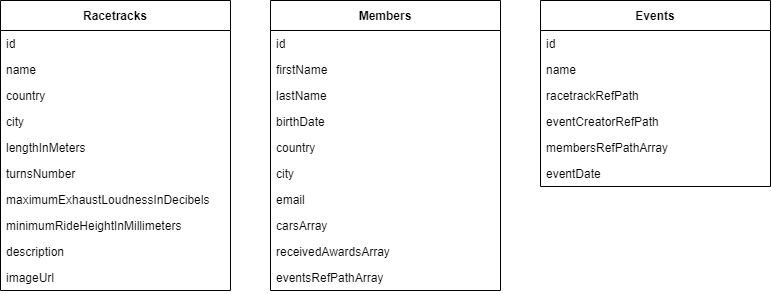
\includegraphics[width=0.85\textwidth, keepaspectratio]
                {img/chapter4/firestore_collection_diagram.png}
                \caption
                [Kolekcje istniejące w bazie danych Cloud Firestore]
                {Kolekcje istniejące w bazie danych Cloud Firestore}
                \label{chapter4:dok_techniczna:implementacja:model_danych:diagram_kolekcji}
            \end{figure}

            Warto dodać, że w~projekcie zostały przyjęte pewne konwencje w nazewnictwie
            wcześniej wspomnianych właściwości dokumentu w~danej kolekcji.
            Przedstawione w~dokumencie znajdujący się w~kolekcji zawiera właściwości
            \textit{carsArray} oraz \textit{receivedAwardsArray}. Są to tablice
            zawierające obiekty klas \textit{Car} oraz \textit{Award}, których
            zawartości strukturalne zostały przedstawione na rysunku
            \ref{chapter4:dok_techniczna:implementacja:model_danych:diagram}.

            \begin{figure}[H]
                \centering
                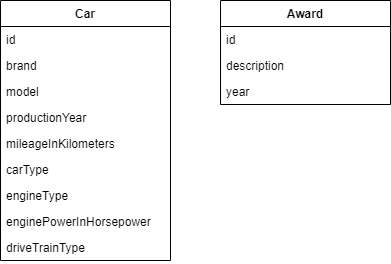
\includegraphics[width=0.45\textwidth, keepaspectratio]
                {img/chapter4/car_award_diagram.png}
                \caption
                [Zawartości strukturalne klas \textit{Car} oraz \textit{Award}]
                {Zawartości strukturalne klas \textit{Car} oraz \textit{Award}}
                \label{chapter4:dok_techniczna:implementacja:model_danych:diagram}
            \end{figure}

            Kolejną sprawą jest łączenie naturalnie powiązanych ze sobą dokumentów
            z~różnych kolekcji. Zgodnie z~zaprezentowanymi w~oficjalnej dokumentacji
            technicznej bazy danych Cloud Firestore technikami zostały stworzone
            właściwości w~dokumentach wybranych kolekcji odpowiadające za
            przechowywania odniesień do dokumentów z~innych kolekcji. W~zależności od
            tego czy przechowują jedno odniesienie czy też wiele posiadają sufiks
            odpowiednio \textit{RefPath} lub \textit{RefPathArray}. Przykładem
            zawartość właściwości przechowującej odniesienie \textit{eventCreatorRefPath}
            do innego dokumentu z~innej kolekcji jest przedstawiony ciąg tekstowy dla
            \shellcmd{/members/j1VVqMXuoNefURvUVjyE53OMtFm1}. Odnosi się ona do
            dokumentu z~kolekcji \shellcmd{Members} o~ID
            \shellcmd{j1VVqMXuoNefURvUVjyE53OMtFm1} .

            Do przechowywania plików binarnych, takich jak zdjęcia jest wykorzystywane
            Firestore Storage. Moduł ten został opisany w~sekcji
            \ref{chapter3:technologie:firebase:storage}.
            Sama baza danych przechowuje jedynie URL do danych plików i~pobranie go
            w~przypadku potrzeby jest wykonywane poprzez Storage SDK, które zostało
            opisane w~sekcji \ref{chapter3:technologie:firebase:storage}. Zgodnie
            z~przyjętą konwecją właściwość dokumentu w~danej kolekcji jest oznaczana
            poprzez sufiks \textit{Url} i~przykładem takiej właściwości jest
            \textit{imageUrl} w~dokumentach kolekcji \textit{Racetracks}.
        }

        \subsection{Warstwa obsługi interfejsu programistycznego aplikacji API}
        \label{chapter4:dok_techniczna:implementacja:api} {
            Ze względu na dosyć nowatorskie rozwiązanie obsługi bazy danych poprzez
            zapewnienie metod znajdujących się w~SDK poszczególnych produktów
            wchodzących w~skład platformy Firebase, które zostały opisane w~sekcjach
            \ref{chapter3:technologie:firebase:firestore},
            \ref{chapter3:technologie:firebase:storage},
            \ref{chapter3:technologie:firebase:functions} w~aplikacja została stworzona
            warstwa logiki, która znajduję się w~folderze \textit{logic}. Jej zadaniem
            jest opakowanie metod oraz funkcji zapewnione przez SDK. Pierwszą podwarstwą
            jest warstwa ogólna zawierająca wszystkie metody dostępne w~SDK natomiast
            kolejną podwarstwą są skonkretyzowane dla danej kolekcji metody. Ułatwia to
            użycie, zwiększa czytelność kodu oraz zmniejsza ilość nadmiarowego kodu
            gdyż nie jest on nigdzie powtórzony a~jedynie są wywołania funkcji czy też
            metod w~wielu komponentach biblioteki React, która została opisana w~sekcji
            \ref{chapter3:technologie:react}. Aby podążać w~sposób konsekwentny
            w~nazewnictwie każda taka klasa zawierająca takie metody czy też plik
            z~funkcjami posiada sufiks \textit{Controller} natomiast skonkretyzowane
            użycie zawiera w~nazwie prefiks kolekcji w~formie pojedynczej na przykład
            \textit{Racetrack}. Mało skomplikowanym choć obrazującym w~bardzo dobry
            sposób jest przykład użycia Firebase Storage,
            \textit{FirebaseStorageController}, który należy do warstwy ogólnej oraz
            \textit{RacetrackFirebaseStorageController}, który z~kolei należy do
            skonkretyzowanej warstwy. Tak jak zostało to przedstawione na listingu
            \ref{chapter4:dok_techniczna:implementacja:api:generic}, jest to opakowanie
            we własne metody, funkcji zapewnionych przez SDK. Na listingu
            \ref{chapter4:dok_techniczna:implementacja:api:concrete} zostały
            przedstawione konkretne ich użycia uwzględniające założenia logiczne
            aplikacji oraz przenoszące część odpowiedzialności na te metody a~nie
            bezpośrednio na ich wywołanie. Przykładem takiego zabiegu jest chociażby
            konkretyzacja ścieżki (ang. path) oraz typu przesyłanych danych. Warto
            dodać, że ze względu na mnogość dostępnych metod w~SDK zostały
            przedstawione niepełne listingi omówionych klas.

            \begin{code}[H]
                \lstinputlisting{../listing/chapter4/api_generic_controller.txt}
                \caption
                [Kod źródłowy klasy FirebaseStorageController]
                {Kod źródłowy klasy FirebaseStorageController}
                \label{chapter4:dok_techniczna:implementacja:api:generic}
            \end{code}

            \begin{code}[H]
                \lstinputlisting{../listing/chapter4/api_concrete_controller.txt}
                \caption
                [Kod źródłowy klasy RacetrackFirebaseStorageController]
                {Kod źródłowy klasy RacetrackFirebaseStorageController}
                \label{chapter4:dok_techniczna:implementacja:api:concrete}
            \end{code}
        }

        \subsection{Struktura stron}
        \label{chapter4:dok_techniczna:implementacja:struktura_stron} {
            Ze względu na to, że aplikacja \textit{Social Racetrack} została stworzona
            w~koncepcji SPA poprzez użycie biblioteki React nie przeładowywuje
            ona stron. Cały ten koncept i~technologia zostały przedstawione w~sekcji
            \ref{chapter3:technologie:react}. Z~pomocą w~przypadku potrzeby posiadania
            wielu stron przychodzi biblioteka \textit{React Router Dom}. Zapewnia ona
            możliwość ładowania określonych komponentów ze względu na adres URL, co
            zapewnia symulację podziału aplikacji internetowej na strony. Poniżej zostały
            przedstawione adresy URL i~odpowiadające mu komponenty. Zostały one
            podzielone ze względu na poziom wymaganych uprawnień aby mieć do nich dostęp.

            \subsubsection{Komponenty dostępne publicznie}
            \label{chapter4:dok_techniczna:implementacja:struktura_stron:publiczne} {

                \noindent\textbf{https://domena/login}\\
                \indent Komponent \textit{LoginPage}, którego zadaniem jest wyświetlanie
                panelu logowania. Został on przedstawiony na rysunku
                \ref{chapter5:dok_uzytkownika:logowanie_rejestracja:login_panel}.

                \noindent\textbf{https://domena/reset-password}\\
                \indent Komponent \textit{ResetPasswordPage}, którego zadaniem jest
                wyświetlanie panelu przywracania hasła. Został on przedstawiony na
                rysunku
                \ref{chapter5:dok_uzytkownika:logowanie_rejestracja:reset_password}.

                \noindent\textbf{https://domena/register}\\
                \indent Komponent \textit{RegisterPage}, którego zadaniem jest wyświetlanie
                panelu rejestracji użytkownika. Został on przedstawiony na rysunku
                \ref{chapter5:dok_uzytkownika:logowanie_rejestracja:register_panel}.

                \noindent\textbf{https://domena/}\\
                \indent Komponent \textit{HomePage}, którego zadaniem jest wyświetlanie
                głównej strony. Został on przedstawiony na rysunku
                \ref{chapter5:dok_uzytkownika:wprowadzenie_interface:ui_intro}.

                \noindent\textbf{https://domena/racetracks}\\
                \indent Komponent \textit{RacetracksPage}, którego zadaniem jest
                wyświetlanie obiektów sportowych. Został on przedstawiony na rysunku
                \ref{chapter5:dok_uzytkownika:obsluga_niezalogowany:racetracks}.

                \noindent\textbf{https://domena/racetrack-details}\\
                \indent Komponent \textit{RacetrackDetailsPage}, którego zadaniem jest
                wyświetlanie szczegółów obiektów sportowych. Został on przedstawiony
                na rysunku
                \ref{chapter5:dok_uzytkownika:obsluga_niezalogowany:racetrack_details}.
            }

            \subsubsection{Komponenty dostępne dla zalogowanego użytkownika}
            \label{chapter4:dok_techniczna:implementacja:struktura_stron:zalogowany} {

                \noindent\textbf{https://domena/account}\\
                \indent Komponent \textit{AccountPage}, którego zadaniem jest wyświetlanie
                profilu użytkownika. Został on przedstawiony na rysunku
                \ref{chapter5:dok_uzytkownika:funkc_uzyt_zalog:user_panel}.

                \noindent\textbf{https://domena/account-settings}\\
                \indent Komponent \textit{AccountSettingsPage}, którego zadaniem jest
                zapewnienie możliwość dodawania pojazdów, osiągnięć sportowych oraz edycja
                danych osobistych użytkownika. Wszystkie te możliwości został
                przedstawione na rysunkach
                \ref{chapter5:dok_uzytkownika:funkc_uzyt_zalog:add_car},
                \ref{chapter5:dok_uzytkownika:funkc_uzyt_zalog:add_award},
                \ref{chapter5:dok_uzytkownika:funkc_uzyt_zalog:edit_user_data}.

                \noindent\textbf{https://domena/create-event}\\
                \indent Komponent \textit{CreateEventPage}, którego zadaniem jest
                wyświetlanie panelu tworzenia wydarzeń. Został on przedstawiony na rysunku
                \ref{chapter5:dok_uzytkownika:funkc_uzyt_zalog:tworz_wydarz:create_event}.

                \noindent\textbf{https://domena/future-events}\\
                \indent Komponent \textit{FutureEventsPage}, którego zadaniem jest
                wyświetlanie przyszłych wydarzeń. Został on przedstawiony na rysunku
                \ref{chapter5:dok_uzytkownika:funkc_uzyt_zalog:przeglad_wydarz:future_events_panel}.

                \noindent\textbf{https://domena/past-events}\\
                \indent Komponent \textit{PastEventsPage}, którego zadaniem jest
                wyświetlanie przeszłych wydarzeń. Jego wygląd jest identyczny w
                stosunku do komponentu odpowiadającego za wyświetlanie przyszłych
                wydarzeń z~wyjątkiem braku możliwości tworzenia wydarzenia.

                \noindent\textbf{https://domena/event-details}\\
                \indent Komponent \textit{EventDetailsPage}, którego zadaniem jest
                wyświetlanie szczegółów wybranego wydarzenia. Został on przedstawiony
                na rysunku
                \ref{chapter5:dok_uzytkownika:funkc_uzyt_zalog:przeglad_wydarz:event_details}.

                \noindent\textbf{https://domena/members}\\
                \indent Komponent \textit{MembersPage}, którego zadaniem jest
                wyświetlanie kont użytkowników aplikacji. Został on przedstawiony na
                rysunku
                \ref{chapter5:dok_uzytkownika:funkc_uzyt_zalog:przeglad_kont:members_panel}.

                \noindent\textbf{https://domena/member-details}\\
                \indent Komponent \textit{MemberDetailsPage}, którego zadaniem jest
                wyświetlanie szczegółów wybranego konta użytkownika aplikacji. Został
                on przedstawiony na rysunku
                \ref{chapter5:dok_uzytkownika:funkc_uzyt_zalog:przeglad_kont:member_details}.
            }

            \subsubsection{Komponenty dostępne dla administratora}
            \label{chapter4:dok_techniczna:implementacja:struktura_stron:admin} {

                \noindent\textbf{https://domena/admin-panel}\\
                \indent Komponent \textit{AdminPanelPage}, którego zadaniem jest
                wyświetlanie panelu administratora. Został on przedstawiony na rysunku
                \ref{chapter5:dok_uzytkownika:funkc_admin:obsl_panel:grant_admin_panel}.

                \noindent\textbf{https://domena/create-racetrack}\\
                \indent Komponent \textit{CreateRacetrackPage}, którego zadaniem jest
                wyświetlanie panelu dodawania obiektu sportowego. Został on przedstawiony
                na rysunku
                \ref{chapter5:dok_uzytkownika:funkc_admin:dod_usun_tor:add_racetrack}.
            }
        }

        \subsection{Struktura komponentów i ich użycie}
        \label{chapter4:dok_techniczna:implementacja:struktura_komponentow} {
            Zgodnie z~dobrymi praktykami sugerowanymi przez twórców biblioteki React
            przedstawionej w~sekcji \ref{chapter3:technologie:react} aplikacja została
            podzielona na komponenty wyłącznie funkcyjne z~użyciem React Hooks. Sam
            podział na komponenty został wykonany w~zgodzie z~zasadą
            \textit{"Jeden komponent, jedna odpowiedzialność"} a~co za tym idzie cała
            hierarchia użycia od najbardziej bazowych komponentów poprzez konkretyzujące
            bazowe do określonych zadań po takie składających się z~wielu komponentów
            niżej w~hierarchii. Jedną z~najważniejszych zasad przyświecających autorowi
            było unikanie powtarzania kodu. Bardzo ważne było też tworzenie atomowych komponentów
            o~prostej odpowiedzialności oraz budowanie całości z~małych fragmentów w celu
            uzyskania skalowalnej i~łatwej w~rozbudowie aplikacji. Struktura hierarchii
            komponentów bazowych została przedstawiona na rysunku
            \ref{chapter4:dok_techniczna:implementacja:struktura_komponentow:util}.
            Następnie na rysunku
            \ref{chapter4:dok_techniczna:implementacja:struktura_komponentow:pages}.
            zostały przedstawione komponenty użyte na wybranych strona, których
            struktura została przedstawiona w~sekcji
            \ref{chapter4:dok_techniczna:implementacja:struktura_stron}. Komponenty,
            które były używane w~wielu komponentach stojących wyżej w~hierarchii oraz
            zróżnicowanych odpowiedzialnościach zostały przedstawione na rysunku
            \ref{chapter4:dok_techniczna:implementacja:struktura_komponentow:rest}.

            \begin{figure}[H]
                \centering
                \begin{minipage}[b]{0.45\textwidth}
                    \centering
                    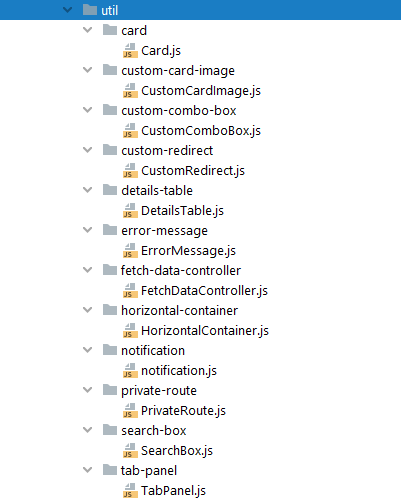
\includegraphics[width=0.85\textwidth, keepaspectratio]
                    {img/chapter4/component_util.png}
                    \caption
                    [Lista komponentów bazowych]
                    {Lista komponentów bazowych}
                    \label{chapter4:dok_techniczna:implementacja:struktura_komponentow:util}
                \end{minipage}
                \hfill
                \begin{minipage}[b]{0.45\textwidth}
                    \centering
                    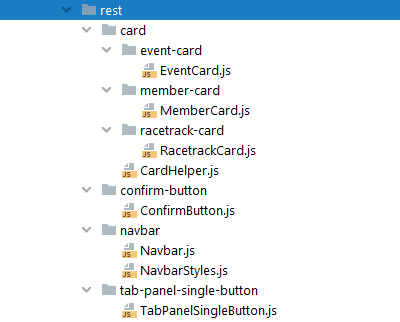
\includegraphics[width=0.85\textwidth, keepaspectratio]
                    {img/chapter4/component_rest.png}
                    \caption
                    [Lista pozostałych komponentów]
                    {Lista pozostałych komponentów}
                    \label{chapter4:dok_techniczna:implementacja:struktura_komponentow:rest}
                \end{minipage}
            \end{figure}

            \begin{figure}[H]
                \centering
                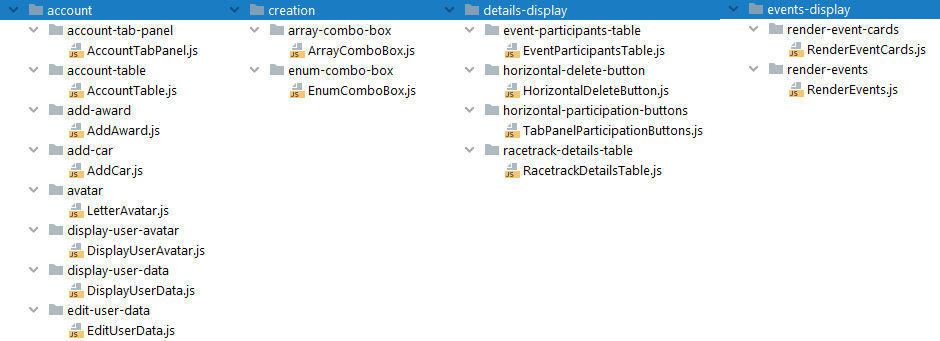
\includegraphics[width=\textwidth, keepaspectratio]
                {img/chapter4/component_pages.png}
                \caption
                [Lista komponentów wykorzystywanych na wybranych stronach]
                {Lista komponentów wykorzystywanych na wybranych stronach}
                \label{chapter4:dok_techniczna:implementacja:struktura_komponentow:pages}
            \end{figure}
        }

        \subsection{Responsywność interfejsu użytkownika}
        \label{chapter4:dok_techniczna:implementacja:responsywnosc} {
            Ze względu na bardzo szeroką gamę urządzeń z~różnymi wymiarami
            i~proporcjami ekranów aplikacja \textit{Social Racetrack} została
            przygotowana z~wykorzystaniem idei RWD, technologii Bootstrap oraz
            projektów rozszerzających jego możliwości, które zostały opisane w~sekcji
            \ref{chapter3:technologie:bootstrap}.

            Świetnym przykładem obrazującym jest strona główna aplikacji przedstawiona
            na rysynku \ref{chapter5:dok_uzytkownika:wprowadzenie_interface:ui_intro}.
            Komponent został podzielony na dwie części, lewą oraz prawą. Ich wyświetlanie
            zostało przedstawione na listingu
            \ref{chapter4:dok_techniczna:implementacja:responsywnosc:rwd_home_page_return_section}
            natomiast fragmenty kodu źródłowego lewej i~prawej części, odpowiednio
            funkcjami \textit{renderLeftSide} oraz \textit{renderRightSide}, zostały
            przedstawione na listingach
            \ref{chapter4:dok_techniczna:implementacja:responsywnosc:rwd_home_page_left_side},
            \ref{chapter4:dok_techniczna:implementacja:responsywnosc:rwd_home_page_right_side}.
            Warto dodać, że fragmenty bezpośrednio nie ilustrujące omawianej tematyki
            w~tej sekcji zostały zastąpione poprzez \shellcmd{//...} .
            Dokładny opis responsywnej siatki został przedstawiony w~sekcji
            \ref{chapter3:technologie:bootstrap:siatka}. Sam podział miejsca na stronie
            został zrealizowany przy wykorzystaniu klasy \textit{col-sm-6}. Oznacza to,
            że do szerokości ekranu \textit{sm} lewa oraz prawa strona będzie zajmować
            cały dostępny ekran. Co do samego ułożenia to najpierw będzie wyświetlona
            lewa część a~pod nia prawa część. Powyżej szerokości \textit{sm} będą one
            zajmować połowę ekranu i~będą umieszczone obok siebie. Definicje rozmiarów
            zostały przedstawione w tabeli
            \ref{chapter3:technologie:bootstrap:siatka:col_size}.

            Co więcej, rozmiar obrazka oraz opisu umieszczonego nad nim zmienia się wraz
            z~rozmiarem ekranu. Zostało użyte połączenie trzech klas
            \textit{col-md-12}, \textit{col-lg-10}, \textit{col-xl-8}. Skutkuje to tym,
            że do szerokość ekranu mniejszej niż \textit{lg} obrazek i~opis zajmuje
            całą dostępna przestrzeń, gdy szerokość ekranu jest z~przedziału klas
            \textit{lg} oraz \textit{xl} to zajmuje 10/12 szerokości ekranu natomiast
            od szerokości \textit{xl} zajmuje 8/12 szerokości ekranu.

            \begin{code}[H]
                \lstinputlisting{../listing/chapter4/rwd_home_page_right_side.txt}
                \caption
                [Kod komponentu HomePage odpowiedzialny za wyświetlanie jej prawej części]
                {Kod komponentu HomePage odpowiedzialny za wyświetlanie jej prawej części}
                \label{chapter4:dok_techniczna:implementacja:responsywnosc:rwd_home_page_right_side}
            \end{code}

            \begin{code}[H]
                \lstinputlisting{../listing/chapter4/rwd_home_page_left_side.txt}
                \caption
                [Kod komponentu HomePage odpowiedzialny za wyświetlanie jej lewej części]
                {Kod komponentu HomePage odpowiedzialny za wyświetlanie jej lewej części}
                \label{chapter4:dok_techniczna:implementacja:responsywnosc:rwd_home_page_left_side}
            \end{code}

            \begin{code}[H]
                \lstinputlisting{../listing/chapter4/rwd_home_page_return_section.txt}
                \caption
                [Sekcja odpowiedzialna za łączenie lewej i prawej części komponentu HomePage]
                {Sekcja odpowiedzialna za łączenie lewej i prawej części komponentu HomePage}
                \label{chapter4:dok_techniczna:implementacja:responsywnosc:rwd_home_page_return_section}
            \end{code}
        }
    }

    \section{Instalacja}
    \label{chapter4:dok_techniczna:instalacja} {
        W celu dokonania procesu instalacji należy na lokalnej maszynie posiadać
        zainstalowane środowisko uruchomieniowe Node.js, które zostało opisane w sekcji
        \ref{chapter3:technologie:node}, menadżer pakietów Yarn przedstawiony w~sekcji
        \ref{chapter3:technologie:node:yarn} oraz należy posiadać zaktualizowaną
        przeglądarkę internetową. Zalecanymi są Chrome\cite{website:chrome} lub
        Firefox\cite{website:firefox} ze względu na dużą popularności oraz wsparcie
        dla nowoczesnych technologii. Kluczowy jest również dostęp do sieci Internet,
        bez którego instalacja nie zakończy się sukcesem.

        Pierwszym krokiem jest uzyskanie dostępu do kodu źródłowego aplikacji
        i~umieszczenie go w~wybranej lokalizacji na wcześniej wspomnianej lokalnej
        maszynie. Kolejnym krokiem jest uruchomienie przeglądarki i~uruchomienie strony
        pod adresem \\ \url{https://console.firebase.google.com/} . Następnie należy
        utworzyć lub zalogować się na konto \textit{Google} i~w~konsoli platformy
        chmurowej Firebase opisanej w~sekcji \ref{chapter3:technologie:firebase}
        stworzyć nowy projekt poprzez przejście konfiguratora projektu i~nadanie mu
        nazwy. Po wykonaniu tej czynności powinien być dostępny projekt ze wszystkimi
        darmowymi usługami.

        Następnym ważnym krokiem, który należy wykonać na maszynie lokalnej jest
        otwarcie konsoli i~przejście do lokalizacji w~której jest umieszczony kod
        źródłowy oprogramowania. Następnie należy wykonać komendę
        \shellcmd{yarn install} , później trzeba przejść do katalogu \textit{functions}
        korzystając z~poleceń charakterystycznych dla danego systemu operacyjnego oraz
        wykonać polecenie \shellcmd{npm install} . Następny z~kolei krokiem jest powrót
        do głównego katalogu w kodzie źródłowym aplikacji i~wykonanie komend
        \shellcmd{npm install -g firebase-tools} oraz \shellcmd{firebase login}
        odpowiadających kolejno za globalną instalacje pakietu \textit{firebase-tools}
        oraz za zalogowanie do konta Google korzystając adresu email oraz hasła
        z wcześniej utworzonego konta. Kolejnym zadaniem jest powrót do otwartej
        przeglądarki z Firebase Console i~przejście do sekcji ustawień a~następnie do
        karty \textit{Ogólne} i~przewinięcie strony do jej końca w celu pozyskania
        kluczy projektu, które należy zgodnie z~przedstawioną instrukcją na stronie
        umieścić w pliku \textit{.env}. Zapewnienie błędnych kluczy lub pomyłka w~ich
        kolejności skutkuję niepowodzieniem w~instalacji.

        Kolejnym krokiem jest określenie sposób autentykacji użytkowników aplikacji.
        Należy wybrać z~bocznego panelu kartę \textit{Authentication}, przejść do karty
        \textit{Sign-in method} a~następnie aktywować aktywować autentykacji poprzez
        \textit{email/haslo}.

        Następnie należy uruchomić polecenie, którego zadaniem jest udostępnienie zasad
        dostępu do bazy danych Cloud Firestore opisanej w~sekcji
        \ref{chapter3:technologie:firebase:firestore} poprzez polecenie
        \shellcmd{firebase deploy --only firestore:rules} lub skorzystanie ze
        skryptu uruchamianego poleceniem \shellcmd{yarn fb:db} .

        Następnym krokiem jest udostępnienie zasad dostępu do Firebase Storage
        opisanego w~sekcji \ref{chapter3:technologie:firebase:storage}. Należy tego
        dokonać poprzez wykonanie polecenie
        \shellcmd{firebase deploy --only storage:rules} lub użycie skryptu uruchamianego
        poleceniem \shellcmd{yarn fb:stor} .

        W~celu udostepnienia funkcji serwerowych określonych mianem Cloud Functions
        przedstawionych w~sekcji \ref{chapter3:technologie:firebase:functions} należy
        wykonać polecenie \shellcmd{firebase deploy --only functions} lub skorzystać ze
        skrypty uruchamianego poleceniem \shellcmd{yarn fb:fun} .

        Ostatecznym krokiem jest udostępnienie aplikacji w~sieci Internet. Aby tego
        dokonać należy skorzystać z~poleceń \shellcmd{yarn build} oraz
        \shellcmd{firebase deploy --only hosting} lub użyć skryptu uruchamianego
        poleceniem \shellcmd{yarn fb:host} .
    }
}
\end{document}
